\section{1D Burger Equation Datasets}

\begin{secframe}
\small
\textcolor{red_unipd}{\Large Dataset Generation for 1D Burger Equation}

\vspace{0.6em}

\begin{block}{Datasets description}
\begin{itemize}
    \item We generated datasets for different viscosity values $\epsilon$.
    \item Changing the value of viscosity has an effect on the smoothness and sharpness of the solution as it evolves.
    \item We consider four datasets with $\epsilon = \{0.001, 0.01, 0.1, 0.5\}$.
    \item The higher the value of $\epsilon$, the smoother the solution is over time.
\end{itemize}
\end{block}

\end{secframe}

% ===== Dataset ε = 0.01 =====
\begin{secframe}

\begin{block}{Dataset 1: $\epsilon = 0.01$}
\begin{itemize}
  \item \small The solutions develop steep gradients rapidly.
  \item \small Not full discontinuities, but sharper transitions.
  \item \small Weak diffusion pattern.
\end{itemize}
\end{block}

\begin{figure}[h!]
    \centering
    \begin{minipage}[t]{0.48\linewidth}
        \centering
        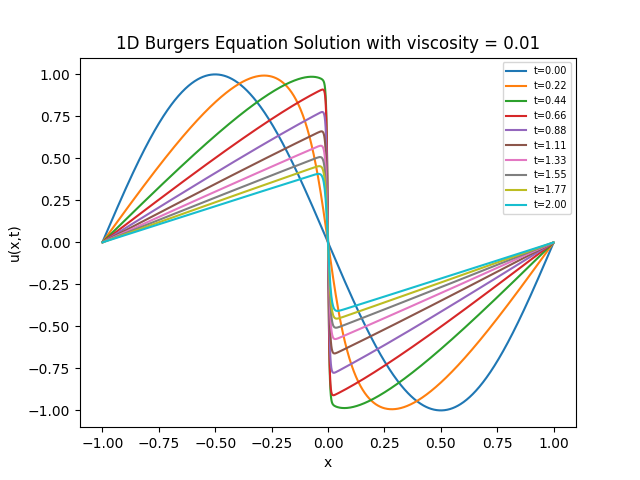
\includegraphics[height=3.7cm]{images/graphical_visualization_1DBurgers_visc_001.png}
    \end{minipage}\hfill
    \begin{minipage}[t]{0.48\linewidth}
        \centering
        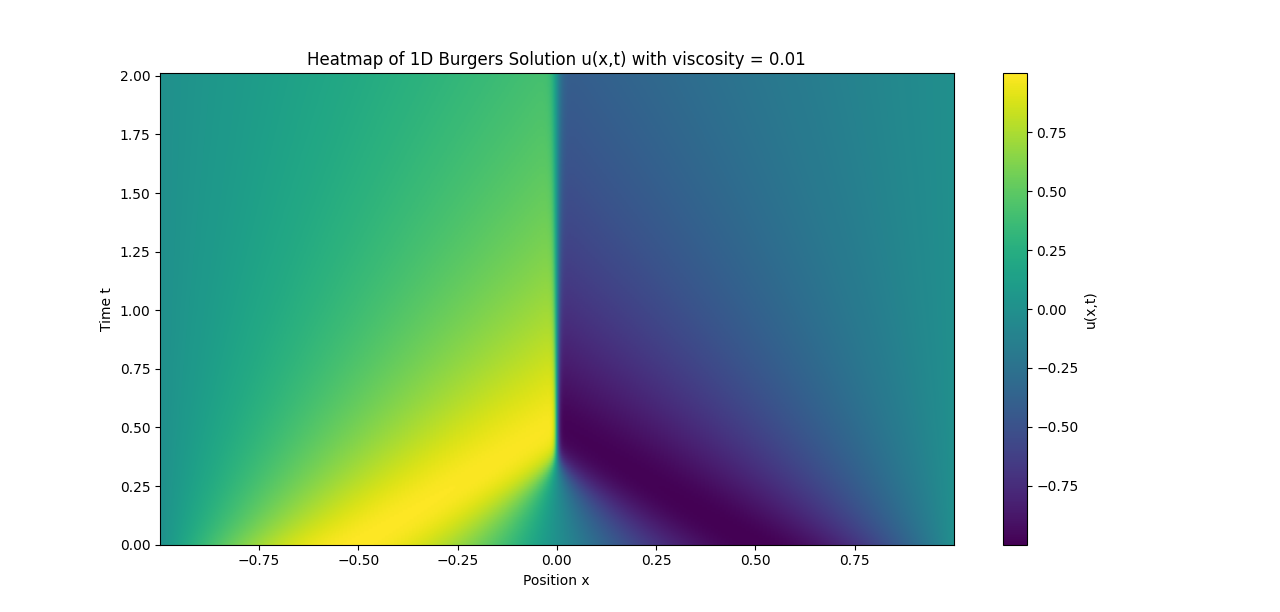
\includegraphics[height=3.7cm]{images/Heatmap_1DBurgers_visc_001.png}
    \end{minipage}
    \caption{\scriptsize Left: solution $u(x,t)$ for 10 different time snapshots; Right: heatmap of $u(x,t)$ evolution.}
\end{figure}

\end{secframe}

% ===== Dataset ε = 0.001 =====
\begin{secframe}
\begin{block}{Dataset 2: $\epsilon = 0.001$}
\begin{itemize}
  \item \small Get steeper gradients more quickly.
  \item \small Almost discontinuities forming in the solution.
  \item \small Minimal diffusion patterns.
\end{itemize}
\end{block}

\begin{figure}[h!]
    \centering
    \begin{minipage}[t]{0.48\linewidth}
        \centering
        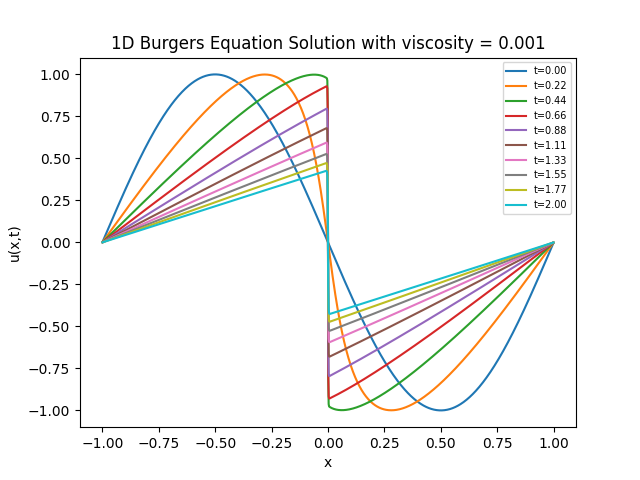
\includegraphics[height=4.0cm]{images/graphical_visualization_1DBurgers_visc_0001.png}
    \end{minipage}\hfill
    \begin{minipage}[t]{0.48\linewidth}
        \centering
        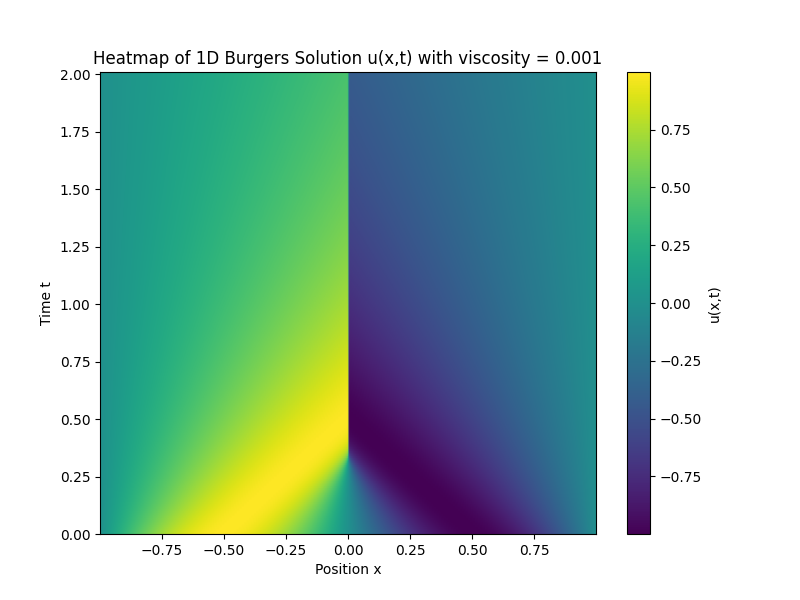
\includegraphics[height=4.0cm]{images/Heatmap_1DBurgers_visc_0001.png}
    \end{minipage}
    \caption{\scriptsize Left: solution $u(x,t)$ for 10 different time snapshots; Right: heatmap of $u(x,t)$ evolution.}
\end{figure}
\end{secframe}

% ===== Dataset ε = 0.1 =====
\begin{secframe}

\begin{block}{Dataset 3: $\epsilon = 0.1$}
\begin{itemize}
  \item \small Higher viscosity leads to smoother solutions.
  \item \small Solutions behave more like a gradually varying wave.
\end{itemize}
\end{block}

\begin{figure}[h!]
    \centering
    \begin{minipage}[t]{0.48\linewidth}
        \centering
        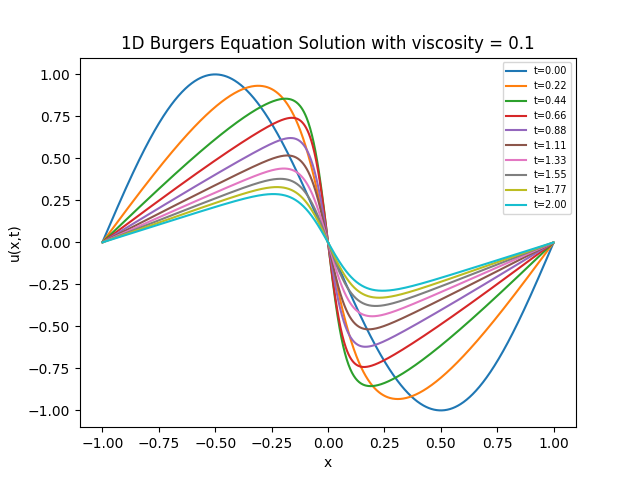
\includegraphics[height=4.0cm]{images/graphical_visualization_1DBurgers_visc_01.png}
    \end{minipage}\hfill
    \begin{minipage}[t]{0.48\linewidth}
        \centering
        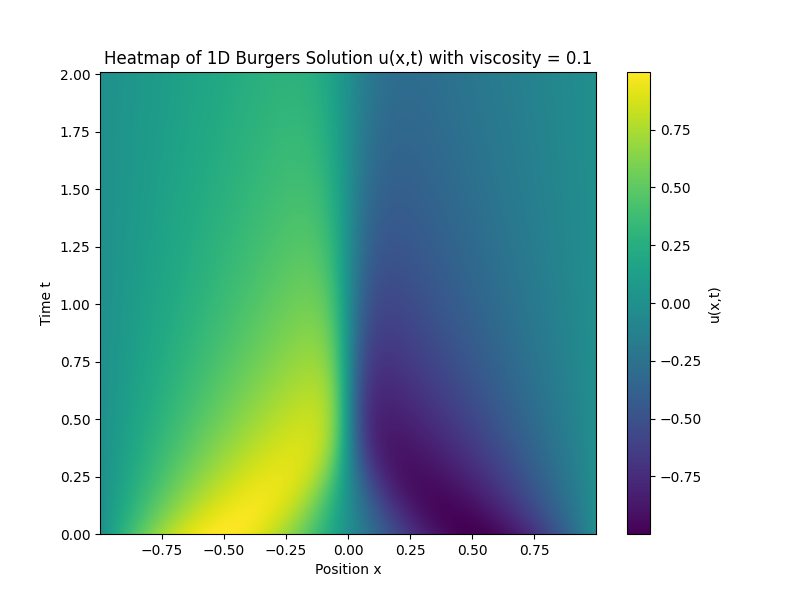
\includegraphics[height=4.0cm]{images/Heatmap_1DBurgers_visc_01.png}
    \end{minipage}
    \caption{\scriptsize Left: solution $u(x,t)$ for 10 different time snapshots; Right: heatmap of $u(x,t)$ evolution.}
\end{figure}

\end{secframe}

% ===== Dataset ε = 0.5 =====
\begin{secframe}

\begin{block}{Dataset 4: $\epsilon = 0.5$}
\begin{itemize}
  \item \small The solution remains smoother over longer times.
  \item \small The solution changes in a smooth way.
  \item \small More diffused patterns. 
\end{itemize}
\end{block}

\begin{figure}[h!]
    \centering
    \begin{minipage}[t]{0.48\linewidth}
        \centering
        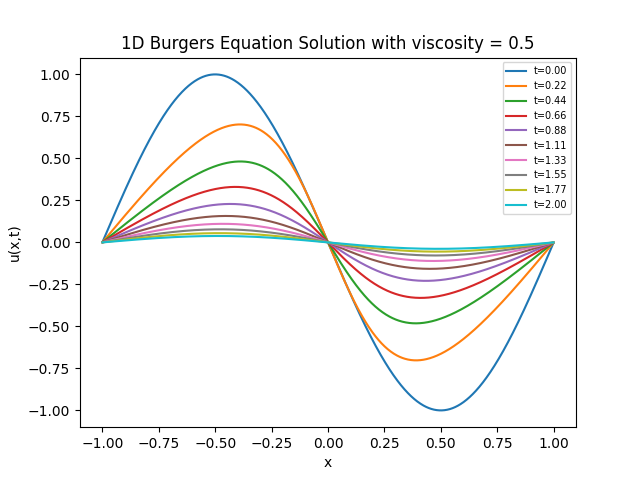
\includegraphics[height=4.0cm]{images/graphical_visualization_1DBurgers_visc_05.png}
    \end{minipage}\hfill
    \begin{minipage}[t]{0.48\linewidth}
        \centering
        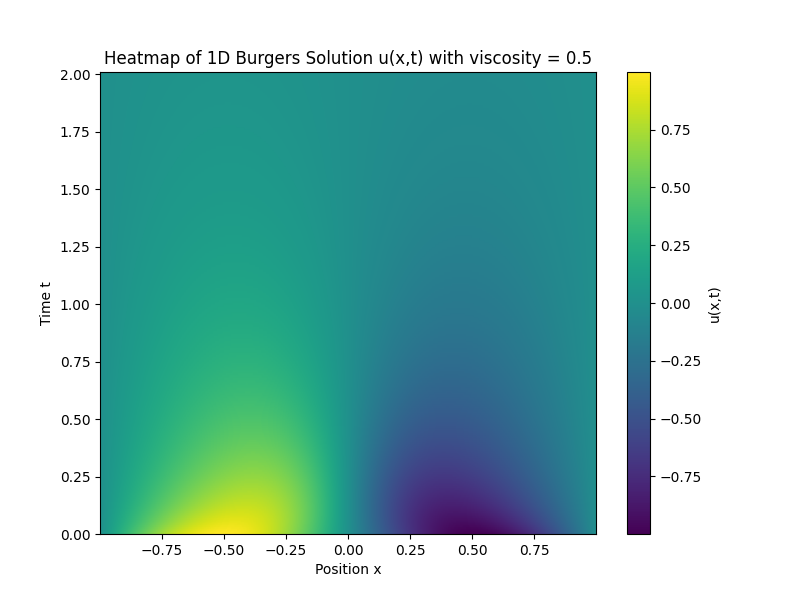
\includegraphics[height=4.0cm]{images/Heatmap_1DBurgers_visc_05.png}
    \end{minipage}
    \caption{\scriptsize Left: solution $u(x,t)$ for 10 different time snapshots; Right: heatmap of $u(x,t)$ evolution.}
\end{figure}
\end{secframe}